\documentclass{article}

\usepackage[utf8]{inputenc}

\usepackage{amsmath}
\newcommand\Rey{\mathrm{Re}}

\usepackage{amsfonts}
\usepackage{amssymb}
\usepackage{outlines}
\usepackage{xcolor}
\usepackage{geometry}
\usepackage{siunitx}

\usepackage{marginnote}
\renewcommand*{\marginfont}{\color{red}\sffamily}

\usepackage{lineno}
\renewcommand\linenumberfont{\normalfont\small\sffamily}
%\linenumbers

\usepackage{graphicx}
\graphicspath{{../pics/}}

\usepackage{natbib}

\begin{document}

\section{Introduction}

\begin{itemize}
    \item Riverine and estuarine sediment budgets play an important role in shaping aquatic and riparian geomorphology and plant communities, particularly in low-gradient coastal landforms (e.g., river deltas).
    \item In turn, plants can affect patterns of erosion and deposition via several mechanisms, one of the less well-understood being direct particle capture by submerged stems, leaves, and other surfaces (Figure \ref{fig:capeff}). 
    \begin{figure}[htbp]
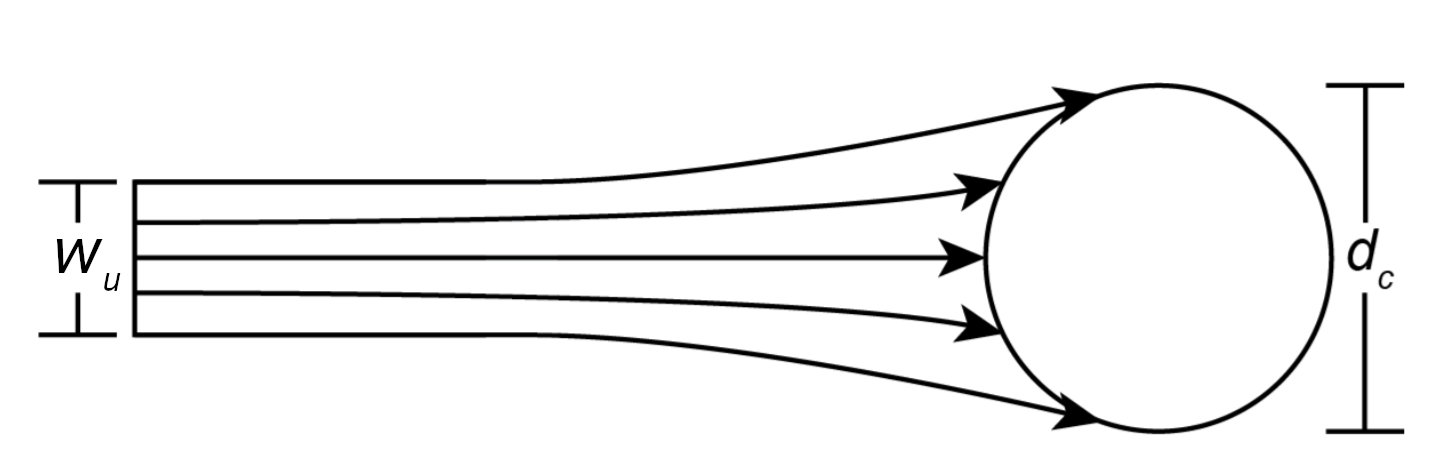
\includegraphics[width=10cm]{collectorefficiency.png}
\centering
\caption{A diagram illustrating capture efficiency for a cylindrical collector. $b$ is the horizontal width of upstream flow and $d_c$ is collector diameter. Adapted from \cite{Palmer_2004}.}
\label{fig:capeff}
\end{figure}
    \item Many previous studies have used laboratory flume experiments to examine the effects of different flow and vegetation conditions on the rate and efficiency of sediment removal from the water column.
    \item Researchers have shown that vegetation stem dimensions, spatial density, and Reynolds number are important predictors of sediment transport and deposition behavior, with analytic expressions derived from fluid dynamics principles informing the case of creeping flow, but no consensus on the nature of these relationships in transitionally turbulent flows. 
    \item Turbulence affects particle capture rates and efficiency, and is also theorized and empirically confirmed to affect other elements of sediment transport behavior, with one particularly important example being its effect on settling velocity.
    \item \cite{Palmer_2004} introduced a power law expression for estimating capture efficiency of cylindrical collectors in transitional turbulence, which takes the form 
        \begin{equation}
            \eta=C{\Rey_c}^{a}R^{b}\,.
            \label{eq:powerlaw}
        \end{equation}
    \item \cite{Fauria_2015} used the same equation form but estimated coefficients using an array of many collectors as opposed to a single one, thereby arriving at a negative relationship between $\eta^\prime$ and $\Rey$ in contrast to the positive relationship between $\eta$ and $\Rey$ found by \cite{Palmer_2004}; this is a major motivator for our study. 
    \item Other motivators include expanding the parameter space to lower collector density, incorporating direct measurement of settling rates to refine capture estimates, and testing replicability and robustness of previous results across different laboratory environments.
    \item \textcolor{violet}{Do you think we should add a paragraph formally stating "we hypothesize...", or would that be redundant with the previous two paragraphs on motivations?}
\end{itemize}

\section{Methods}

\subsection{Suspended Concentration Model}

\begin{itemize}
    \item We used a model adapted from \cite{Fauria_2015} to estimate collection efficiency based on exponential decay of suspended sediment concentration:

\begin{equation}
    \frac{d\bar{\phi}}{dt} = -\left[\frac{Cv_s}{h}(1-E_r) + \eta^{\prime}ud_cI_c\right]\bar{\phi}(t) = -k\bar{\phi}(t)\,.
    \label{eq:model}    
\end{equation}
    This paragraph is a synopsis of the terms of that equation, pointing to \cite{Fauria_2015} for more in-depth derivations, and going into some depth on how we arrive at collector efficiency from the suspended concentration differential equation:
    \begin{equation}
\frac{d\bar{\phi}}{dt} = \frac{N_c}{V}\frac{dN_p}{dt} = \frac{N_c}{V}\eta^{\prime}ud_ch\bar{\phi} = \eta^{\prime}ud_cI_c\bar{\phi}\,.
\label{eq:collection}
\end{equation}
\item Because we assume the vertical profile of sediment concentration maintains a constant shape through time, governed by the Rouse equation, concentration at any height ($\phi_a$) can be assumed to be proportional to average concentration ($\phi_a=\frac{\bar{\phi}}{C}$):
\begin{equation}
    \phi_a(t) = \phi_a(0)e^{-kt}\,,
    \label{eq:specconc}
\end{equation}
which is the formula we used to estimate total time-decay of suspended concentration from our point measurements in the vertical profile.
\item Because sediment likely settled outside the test section, where flow conditions were not controlled, a background factor was included in the decay term ($k = k_c + k_s + k_{bg}$), which was estimated by measuring settling and suspended sediment decay rates in control runs with no collectors ($k_c = 0$).
\end{itemize}

\subsection{Experimental Methods}

\subsubsection{Materials}

\begin{itemize}
    \item Our experiment was conducted in a recirculating flume: water was propelled by an electric pump through a pipe of gradually increasing hydraulic diameter with a rectangular cross-section, through a honeycomb flow collimator, into a rectangular open channel containing our test section, then through another similar pipe feeding back to the pump (Figure \ref{fig:floorplan}).
    \begin{itemize}
        \item channel depth: 40 cm, channel width: 60 cm, and test-section length: 2 m.
    \end{itemize}
    \item Our pump operated without cavitation in its chambers above 30 Hz, which corresponded to a flow velocity of 6 cm/s in the test section; we selected 10, 20, and 30 Hz as our velocity treatment levels to cover a suitable range of Reynolds numbers (67-200), and determined that flow velocity scaled linearly with pump frequency (Figure \ref{fig:freqvel}).
    \begin{itemize}
        \item \textcolor{violet}{Should this figure be cut? I kind of think so.}
    \end{itemize}

\begin{figure}[htbp]
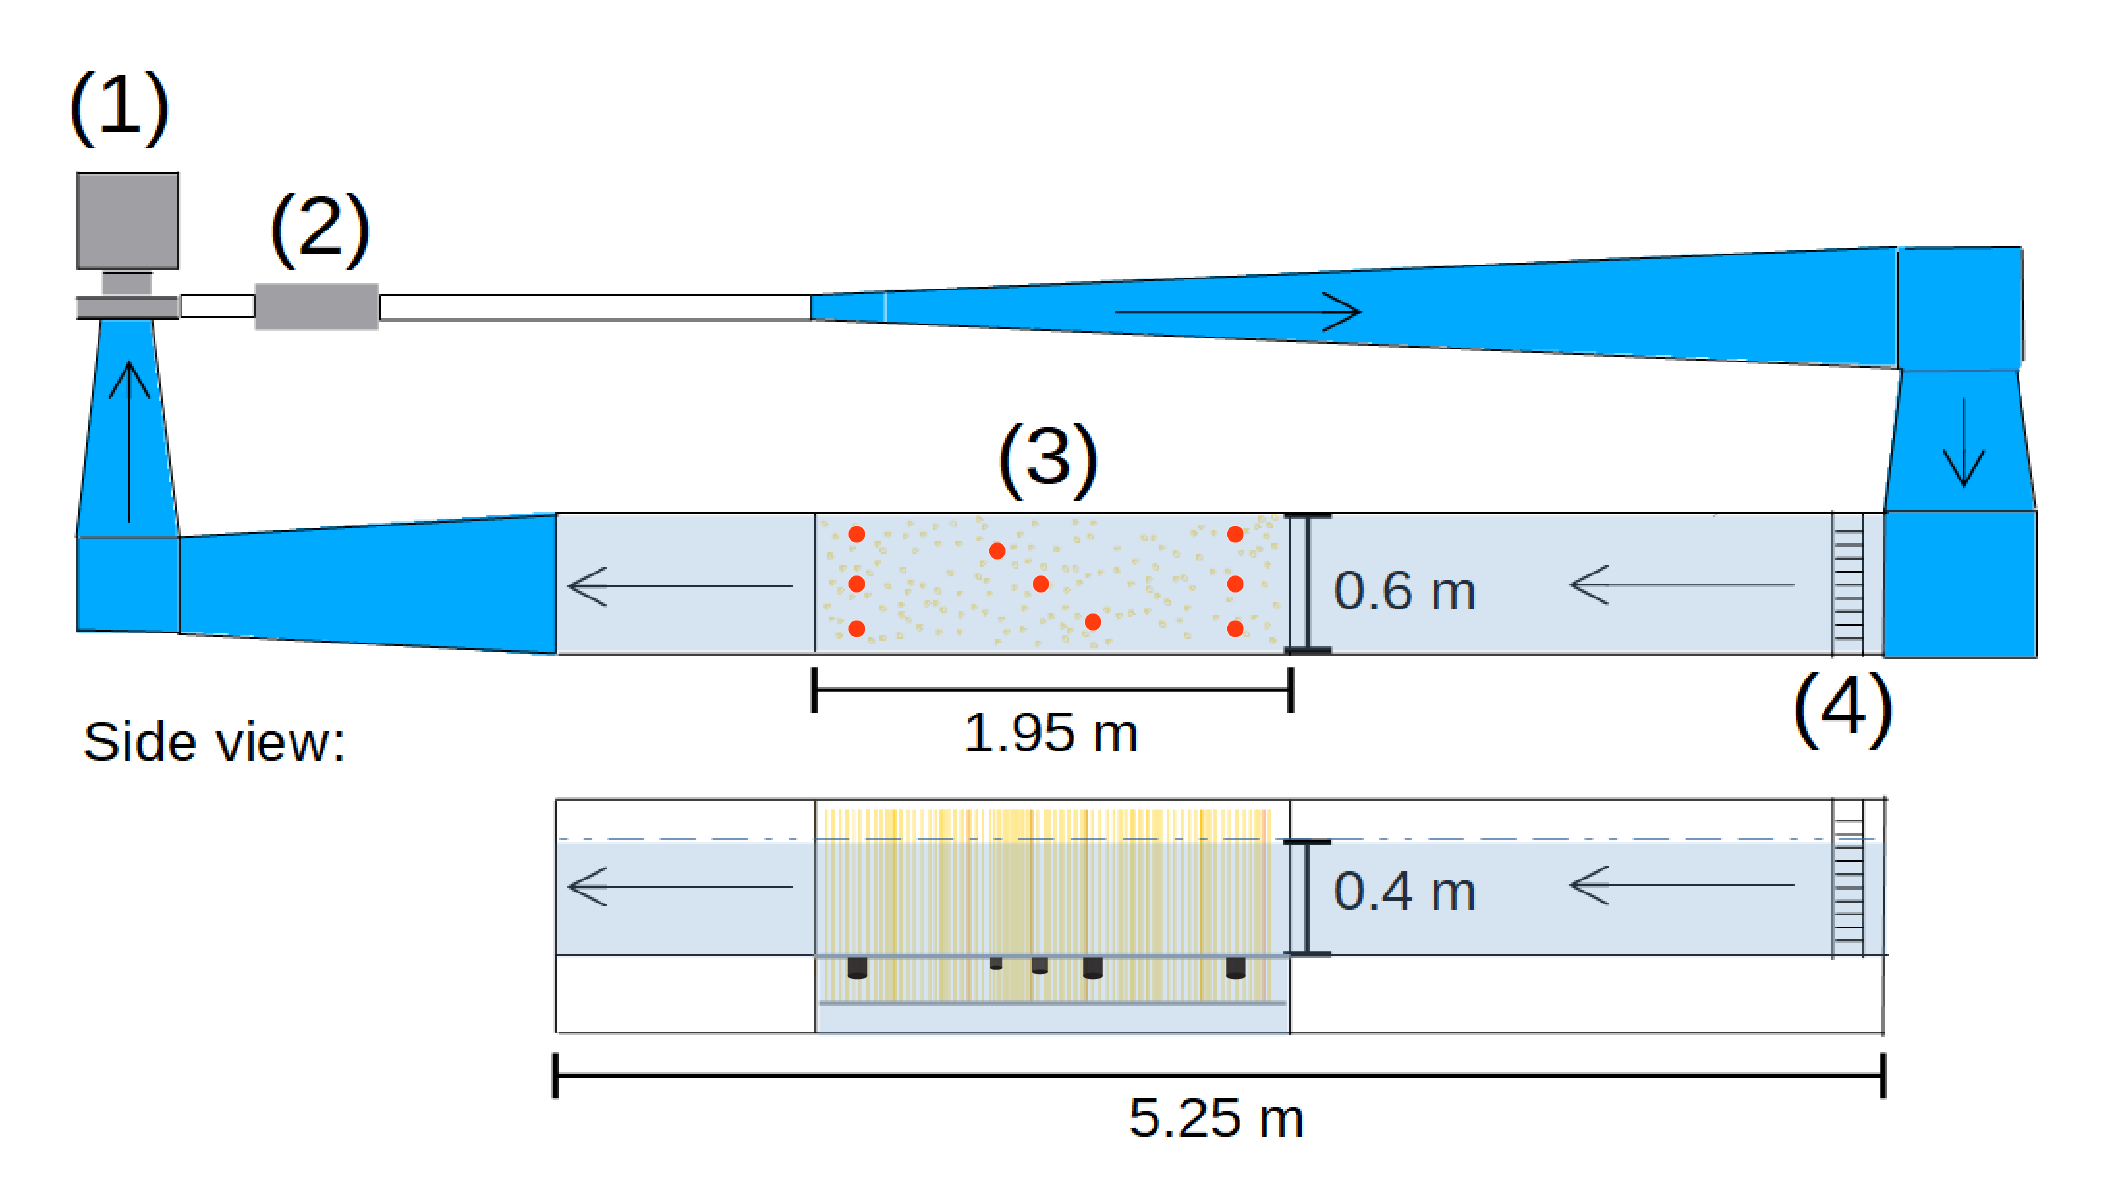
\includegraphics[width=15cm]{../pics/flume_with_sedtraps.png}
\centering
\caption{Conceptual diagram of the laboratory flume. Labeled parts are: 1) pump, 2) magnetic flowmeter, 3) test section, and 4) honeycomb flow collimator. Arrows indicate direction of flow. A side view of the open-channel part of the system is included. Some dimensions not to scale. Red circles in the top-down view and black rectangles in the side view of the test section show the locations of the sediment traps.}
\label{fig:floorplan}
\end{figure}

\begin{figure}[htbp]
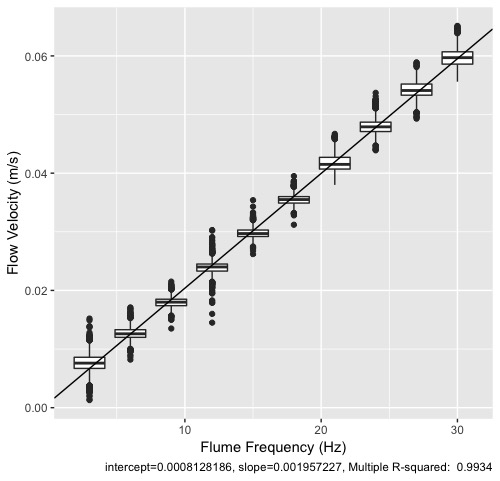
\includegraphics[width=15cm]{frequency_velocity_boxplots.jpeg}
\centering
\caption{Results from the experiment in which we used an acoustic doppler velocimeter (ADV) to determine flow rates in the test section across our pump's span of frequencies without cavitation.}
\label{fig:freqvel}
\end{figure}

    \item We used 1/8" wooden dowels ($d_c = \SI{.3175}{\centi\metre}$) as collector stems, which were greased with silicone (Chemplex 710), and installed in a removable array that filled a recessed well in the bottom of the rectangular channel at densities between 200 and 1500 stems/$\SI{}{\metre^2}$.
    \begin{itemize}
        \item \textcolor{violet}{Should there be a separate section about how we selected parameter values? It kind of seems unclear whether that would come before or after "Materials" since our pump's constraints and dowel size choice were a factor, but the values are also kind of a statistical decision. We should definitely add a table with our parameter ranges juxtaposed with natural ranges like \cite{Fauria_2015} though, right?}
    \end{itemize}
    \item We measured settling directly using sediment traps (n = 9), constructed by affixing small perforated disks with oven-dried and weighed quantitative glass microfiber (Whatman GF/F) filter papers to the inside of hollow plastic cylinders, which were spaced out evenly throughout the test section (Figure \ref{fig:floorplan}). Filters were oven- dried and weighed before and after runs.
    \item We chose to use granular walnut shell flour to simulate sediment for our experiments because it's available in pre-measured sieve size categories, of which we selected WF5-200 grade as the closest match to the natural range of suspended sediment in rivers (Figure \ref{fig:sedsize}).
 \begin{figure}[htbp]
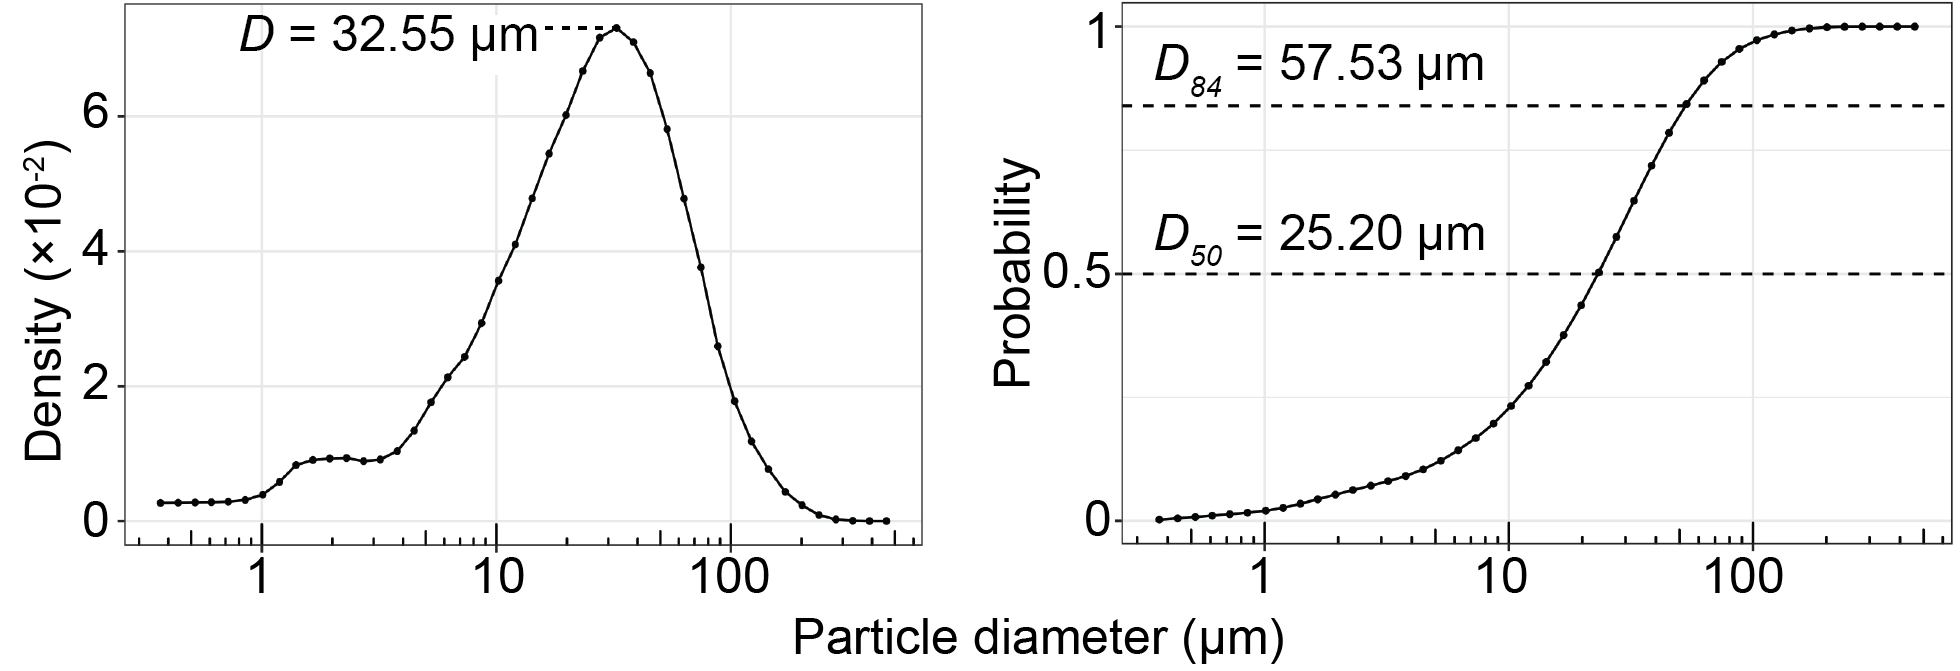
\includegraphics[width=15cm] {wf5-200sizedist.png}
\centering
\caption{Particle size distribution of WF5-200 walnut shell flour used as sediment in experiments, expressed as a probability density function (left) and cumulative density function (right). The mode of the distribution (left) and the 50th and 84th percentiles (right) are labeled.} 
\label{fig:sedsize}
\end{figure}
   




\end{itemize}

\subsubsection{Suspended Concentration Run Protocols}

\begin{itemize}
    \item In our preliminary experiments, we determined 100 minutes was the appropriate run length to capture suspended concentration decay across our parameter space of flow velocities and collector densities.
    \item In order to quantify the suspended particle concentration, we sampled water 50 cm upstream and downstream of the test section at regular intervals of 5 minutes throughout the duration of each experiment, using inlets at heights of 5, 14, and 27 cm from the channel bottom regulated by peristaltic pumps to match channel flow velocity. Samples measured approximately 140 ml each, and our sampling frequency resulted in 19 sampling timesteps per experiment, with six samples per timestep.
\end{itemize}

\subsubsection{Turbulence Estimate Protocols}

\begin{itemize}
    \item For each of the 12 combinations of flow velocity and collector density, including the control runs with zero collectors, acoustic doppler velocimetry (ADV) was used to measure velocity in the test section at positions 6.7, 14.8, 24.9 and 36.1 cm above the flume bed, with each measurement lasting at least 300 seconds to capture longer-period fluctuations. ADV uses tracer particles to measure velocity vectors in the longitudinal, lateral, and vertical directions at relatively high frequency (10 Hz).
\end{itemize}

\subsubsection{Flume Volume Estimate Protocol}

\begin{itemize}
    \item The decay rate due to collection ($k_c$) as discussed thus far is that observed for our experimental setup specifically. In order to estimate $\eta$, we need to know the collection rate for water that is being acted upon by the collectors, which requires scaling up by the ratio between the test section volume (1.95 m $\times$ 0.6 m $\times$ 0.4 m = \SI{0.468}{m^3}) and the water volume of the flume as a whole. To calculate the latter, we drained the flume while measuring flow rate at an outlet with constant height over time, performed polynomial regression, and calculated a definite integral. 
\end{itemize}

\subsubsection{Biofouled Runs}

\begin{itemize}
    \item At each collector density, dowels were allowed to remain submerged after a run for several days, with a fluoresecent light on above the flume. Once visible biofilm growth was observed to occur, a run was done at the highest of our Reynolds number treatments (200), for comparison to the identical run in our main experiment with greased collector surfaces.
\end{itemize}

\subsection{Statistical Analyses}

\subsubsection{Settling and Capture}

\begin{itemize}
    \item The mass of sediment settled due to gravity was estimated by removing and oven-drying sediment trap filters after each run, then calculating their difference in mass due to accumulated sediment. This was scaled to the test section as a whole using the ratio between the trap opening's surface area (\SI{4.98e-4}{\metre^2}) and the area of the test section's bed (\SI{1.17}{\metre^2}). 
    \item This total mass of sediment settled in the test section over the course of the run was then used in combination with the rate at which suspended sediment concentration decayed to estimate the decay rate due to settling in the test section specifically:
    \begin{equation}
        k_s = \frac{m_s}{m_0}(\frac{1}{1-e^{-kT}})k
    \end{equation}
\end{itemize}

\subsubsection{Turbulence and Bed Shear Stress}

\section{Results}

\subsection{Effects of Collector Density and Reynolds Number}

\subsection{Effects of Turbulence}

\subsection{Effects of Biofilm}

\section{Discussion}

\begin{itemize}
    \item In agreement with the power law regression ($\eta^\prime = C\Rey^{-1.14}R^{0.65}$) presented by \cite{Fauria_2015}, capture efficiency ($\eta$) has an approximately inverse relationship with Reynolds number, which is in turn directly proportional to velocity ($u$). Looking at the decay model, $\eta \propto k_c/u$, which means that if our measured $k_c$ were constant across treatments, we'd still expect the relationship $\eta \propto Re^{-1}$. Collector density shares the same proportionality ($\eta \propto k_c/I_c$). Based on our error propogation, the uncertainty in our measurements far outweighs any pattern among our $k_c$ estimates. \textcolor{violet}{Most of the magnitude of the observed negative trend in $\eta^\prime$, over both $\Rey$ and $I_c$, is an artifact of the algebra involved in its calculation rather than actual measured differences between our treatments.} 
        \begin{itemize}
            \item  \textcolor{violet}{I think it's important for everyone to be aware of the simple fact described above...I'm surprised it wasn't discussed in \cite{Fauria_2015}, whose results follow the same pattern, though across fewer treatment levels. As a side note, \cite{Purich_2007} had a low-density treatment that defied this pattern (i.e., had lower $\eta$ than higher densities).} 
        \end{itemize}
    \item We found that biofilm increased $k_c$ in comparison to greased dowels for several collector densities at the high Reynolds number treatment, which as I see it presently, challenges the assumption of \cite{Palmer_2004} and \cite{Fauria_2015} that greased dowels have perfect retention.
    \item At our lowest collector density, we got a measurement of collector efficiency ($\approx2\%$) far greater than any from \cite{Fauria_2015} or \cite{Purich_2007}, suggesting that sheltering of collectors probably plays a large role in limiting $\eta^\prime$ for most densities previously tested, especially at low Re ($\approx60$). Maybe to the point that $k_c$ is minimally affected by density above some threshold (maybe below our lowest treatment), which could make $\eta$ inversely proportional thereafter as detailed above.
\end{itemize}

\bibliographystyle{apalike}
\bibliography{refs}

\end{document}
